\chapter{Transaction Fees and EIP-1559}
In this chapter, we're focusing on different economic issues related to blockchain protocols that have a native cryptocurrency.
\section{Recap}
In the previous chapter (chapter 10), we discussed five reasons for caring about cryptocurrencies in the context of blockchain protocols. First, cryptocurrencies are interesting in their own right. Second, having a native currency makes blockchain protocols more versatile and functional. Third, it enables convenient reward mechanisms for contributors to the protocol. Fourth, native currencies can incentivize desired behavior and discourage unwanted actions. Fifth, cryptocurrencies are crucial for proof-of-stake, a more energy-efficient alternative to proof-of-work consensus.\\
This chapter focuses on using a native cryptocurrency to charge for usage, specifically through transaction fees. Transaction fees play a vital role in blockchains, given the finite processing power and block size of these networks.

\section{Transaction Fees and Economic Efficiency}
\subsection{Blockchains and Limited Throughput}
Blockchains, such as Bitcoin and Ethereum, face a fundamental challenge when it comes to transaction processing - limited throughput. This limitation arises due to two main factors: the rate of block production and the block size.\\

In Bitcoin, blocks are produced at an average rate of one block every 10 minutes. Similarly, in Ethereum, new blocks are created approximately every 13 seconds. These time intervals determine how frequently new transactions can be added to the blockchain. While the rate of block production can be adjusted through protocol updates, there are practical constraints to consider.\\

Another critical factor affecting the throughput is the block size. In the past, Bitcoin had a hard limit of one megabyte per block, leading to debates within the community about increasing the block size to accommodate more transactions. Ethereum, on the other hand, measures block size using a concept called "gas," which represents the computational and storage costs of processing a transaction. Each block in Ethereum has a cap on the total gas that can be used, which effectively limits the number of transactions that can fit within a block.\\

These limitations mean that both Bitcoin and Ethereum, like many other blockchain networks, can only process a relatively small number of transactions per unit of time. For example, Bitcoin's throughput is far less than 10 transactions per second, and Ethereum's throughput is less than 20 transactions per second. In comparison, traditional payment networks like Visa can process thousands of transactions per second.\\

\noindent
\textbf{Challenges in Scaling Blockchains: }The restricted throughput in blockchains raises concerns about scalability and widespread adoption. Simply increasing the block size or rate of block production is not a viable solution due to the goal of permissionless consensus and low barriers to entry. All nodes in the network need to be able to process transactions, and this requirement places a limit on the number of transactions per second. To address these challenges, developers and researchers have been working on Layer Two scaling solutions, which aim to enable a significant increase in the number of transactions that can be processed off-chain while still securing the network using the underlying blockchain.\\

Despite the current limitations, it is crucial to maintain a balance between scalability and the core principles of blockchain networks, such as permissionless consensus and low barriers to entry. These principles ensure that anyone can participate in the network and that all nodes contribute to transaction processing. The limited throughput of blockchains like Bitcoin and Ethereum presents a significant challenge to achieving mainstream adoption and scalability. As the demand for blockchain-based transactions continues to grow, addressing these limitations will be critical to realizing the full potential of blockchain technology in various industries.\\

\noindent
\textbf{Competition for Block Space: }Blockchains like Bitcoin and Ethereum have a limited capacity to process transactions due to the rate of block production and the size of each block. For instance, in Bitcoin, blocks are produced approximately every 10 minutes, while in Ethereum, they are produced every 13 seconds. Additionally, both blockchains have a finite cap on the number of transactions that can fit into a block. For example, Ethereum has a hard limit of 15 million gas per block, which is a proxy for computational and storage costs.\\

The limited throughput of these blockchains presents a challenge for handling a large number of transactions. As a result, there is fierce competition among transactions to be included in the blocks. Miners in the case of Bitcoin or validators in the case of Ethereum must decide which transactions to include and which to exclude from each block.\\

Since block space is a scarce resource, it becomes essential to prioritize valuable transactions that bring significant value to their creators. On the other hand, transactions that may be considered spam or have frivolous uses should be excluded to ensure efficient usage of the blockchain.\\

One may wonder how to determine the value of a transaction and whether it should be included in a block. Asking the transaction creators directly may not be effective, as they could overstate the value of their transactions to get them included.\\

The solution to this challenge lies in the use of transaction fees. By charging a non-trivial transaction fee for executing a transaction on the blockchain, the protocol incentivizes users to indicate the value they place on their transactions. Transactions that are genuinely valuable to their creators will be more willing to pay higher transaction fees, while those with less value will be discouraged from spending large fees. In this way, transaction fees act as a screening mechanism, helping prioritize high-value transactions and disincentivizing low-value or frivolous ones. Thus, transaction fees play a vital role in optimizing the use of limited block space and ensuring the economic efficiency of the blockchain network.

\subsection{Importance of Transaction Fees}
Transaction fees play a crucial role in the functioning of blockchain protocols with native cryptocurrencies, such as Bitcoin and Ethereum. These fees serve two primary purposes that are vital for the efficiency and sustainability of the blockchain network.\\

\noindent
\textbf{1. Discouraging Spam and Frivolous Usage}\\
Even if a blockchain protocol had infinite processing power, it would still be essential to impose transaction fees. A very low and nominal fee could be charged per transaction to discourage spam and frivolous usage of the blockchain. Without transaction fees, malicious actors could flood the network with numerous unnecessary transactions, causing congestion and hindering legitimate transactions from being processed promptly.\\

By charging a small fee, blockchain networks can prevent these types of abusive behaviors, making it economically unfeasible for attackers to conduct large-scale spam attacks. This ensures that the blockchain resources are dedicated to genuine and valuable transactions that contribute to the overall functionality and utility of the network.

\noindent
\textbf{2. Prioritizing Valuable Transactions}\\
The limited processing capacity and block size of blockchains pose a challenge in deciding which transactions to include in each block. With a large number of pending transactions at any given time, miners or validators must choose which ones to include in the next block.\\

Transaction fees serve as an incentive mechanism for miners to prioritize certain transactions over others. Transactions that offer higher fees are given preferential treatment, as miners are economically motivated to include them in their blocks. This ensures that transactions with a higher perceived value to their creators are processed promptly.\\

By setting the transaction fees higher for transactions that generate more significant value or have specific urgency, blockchain networks can optimize their throughput and allocate resources more efficiently. This prioritization mechanism aligns intending to maximize the overall utility of the blockchain network.

\subsection{Setting Transaction Fees: User-Suggested and Protocol-Computed}
As we mentioned earlier, transaction fees are a critical component in determining the order in which transactions are included in a blockchain. They serve as an essential mechanism to prioritize valuable transactions while also discouraging spam and frivolous usage of the blockchain. There are two main approaches used to set transaction fees in blockchain protocols with native cryptocurrencies: user-suggested transaction fees and protocol-computed transaction fees.\\

\noindent
\textbf{User-Suggested Transaction Fees}\\
In the user-suggested approach, users themselves can propose the transaction fees they are willing to pay for their transactions to be included in the blockchain. This mechanism is commonly implemented using first-price auctions. Each user attaches a fee to their transaction, indicating the amount they are willing to pay to have their transaction processed quickly.\\

When a new block needs to be created, miners or validators select transactions to include in the block based on the transaction fees offered. Transactions with higher fees are given priority and are more likely to be included in the next block. Users have an incentive to set competitive fees, as they want their transactions to be processed promptly. At the same time, miners or validators are motivated to include transactions with higher fees, as they receive the fees as rewards for processing those transactions.\\

This user-suggested approach has been employed in Bitcoin since its inception and was also used in Ethereum until August 2021. Users have the freedom to decide how much they are willing to pay for their transactions to be processed quickly, which can lead to varying transaction fees based on the urgency of the users' needs.\\

\noindent
\textbf{Protocol-Computed Transaction Fees}\\
An alternative approach to setting transaction fees is to have the protocol itself compute the fees based on predefined rules and conditions. Ethereum's new transaction fee mechanism, known as EIP1559, follows this protocol-computed approach.\\

Under EIP1559, the transaction fees are determined by a formula that takes into account the network's demand and available capacity. The protocol dynamically adjusts the fees based on the congestion in the network. If there is high demand for block space and the network is nearing its capacity, the transaction fees will increase to prioritize transactions. Conversely, when the network is less congested, the fees may decrease, allowing users to enjoy lower transaction costs.\\

The main advantage of protocol-computed transaction fees is that it provides a more predictable and stable fee structure. Users do not need to guess the appropriate fee to set, as the protocol automatically determines the fee based on the current network conditions. Additionally, this approach can lead to a more efficient allocation of block space, ensuring that transactions with higher value or urgency are prioritized during times of high demand.\\

In conclusion, setting transaction fees in blockchain protocols with native cryptocurrencies is crucial for managing limited throughput and encouraging efficient usage of the blockchain. Both user-suggested and protocol-computed approaches have their merits, with user-suggested fees providing flexibility and user choice, while protocol-computed fees offer stability and efficiency in determining fees based on network demand. Each approach caters to different use cases and network requirements, contributing to the overall functionality and scalability of blockchain protocols.

\section{First-Prize Auctions}
In this section, we will explore the most natural and reasonable solution for setting transaction fees in a blockchain protocol: the first price auction. Nakamoto's original proposal for Bitcoin included first price auctions as a transaction fee mechanism, which is still used in Bitcoin to this day. Ethereum also used this mechanism until August 2021 when they switched to a new transaction fee mechanism, which we will discuss later.

\subsection{Introduction}
In a blockchain protocol that uses a first price auction to set transaction fees, users are required to submit their bids along with their transactions. When a user creates a transaction and submits it to the network, they not only provide the necessary information like their digital signature but also include a bid indicating how much they are willing to pay for their transaction to be included in the blockchain and executed.

For example, let's consider a scenario where Alice wants to transfer some native coins from her account $A$ to Bob's account $B$. When Alice initiates the transaction, she will specify the number of coins to be transferred, sign the transaction with her private key, and include a bid denominated in the blockchain's native currency. This bid represents the amount she is willing to pay to have her transaction processed.\\
If Alice's transaction is not selected by any miner to be included in a block, she doesn't have to pay her bid. However, if a miner decides to include her transaction in a block and successfully adds that block to the blockchain, Alice will be required to pay her bid to the miner.\\
Now, the natural question arises: To whom should Alice pay her bid? The answer is straightforward. Since it is the block producer (in a proof of work blockchain, it would be the miner of the block) who decides which transactions to include in the block, it is reasonable for Alice's payment to go to the producer of the block.\\
So, when Alice's transaction is executed and included in a block, the movement of coins specified in her transaction occurs, and additionally, a portion of her coins goes to the miner of that block. This transfer of the transaction fee bid to the block producer is a crucial incentive mechanism that encourages miners to include users' transactions in the blockchain.\\
It's important to note that the transfer of the transaction fee bid to the miner doesn't happen immediately. The bid becomes a valid transfer only when the block in which Alice's transaction is included becomes part of the longest chain. This concept is integral to the security of the blockchain, ensuring that only valid and confirmed transactions are rewarded.\\
Once the block is deeply embedded in the longest chain (often referred to as "confirmed" or having "sufficient confirmations"), the transaction fee bid can be considered permanently transferred to the miner. This confirmation process ensures that other participants in the network recognize the payment and consider the transaction successfully executed.\\

In summary, a first price auction in a blockchain protocol allows users to submit bids along with their transactions. These bids represent the amount users are willing to pay for their transactions to be included and executed in the blockchain. When a miner includes a transaction in a block, the corresponding bid becomes a valid transfer to the miner, incentivizing them to include more transactions and ensuring the security and efficiency of the blockchain.


\subsection{Transaction Execution and Revenue}
When a transaction is executed in a blockchain protocol that uses a first price auction for transaction fees, two important processes occur:

\begin{enumerate}
  \item \textbf{Coin Transfer:} The transaction creator specifies the movement of coins in their transaction. For instance, if a user wants to perform a simple currency transfer, they would include details on how many native coins they want to move from one account to another (e.g., from Account $A$ to Account $B$). This transfer is a fundamental aspect of the transaction's purpose.

  \item \textbf{Transaction Fee Payment:} Along with the transaction details, the creator is also required to provide a bid denominated in the blockchain's native currency. This bid represents the amount the user is willing to pay to have their transaction included in the blockchain and executed. The bid is an incentive for miners, who are responsible for selecting and validating transactions, to prioritize this transaction over others with lower bids.

  \item \textbf{Payment to Miners:} The bid, which is part of the transaction fee, is directed to the miner of the block that includes the transaction. The block producer decides which transactions are added to their block, and by selecting transactions with higher bids, they can maximize their revenue from transaction fees.

  \item \textbf{Conditions for Fee Payment:} It's important to note that the transaction fee is only paid if the transaction is successfully included in a block. If, for any reason, the transaction is not selected to be part of the blockchain (e.g., due to network congestion or low bids), the user is not required to pay the fee.

  \item \textbf{Validation and Confirmation:} In blockchain protocols that utilize a proof-of-work consensus mechanism, such as Bitcoin or Ethereum until August 2021, the validation of transactions and the addition of new blocks occur through mining. Once a block is mined and added to the blockchain, the bids associated with the included transactions become valid and confirmed. However, the bid is considered permanently transferred to the miner only when the block is deeply embedded in the longest chain, usually confirmed by several additional blocks.

  \item \textbf{Impact on Revenue:} The transaction fee revenue is additive with the block reward revenue for the block producer. The block reward consists of newly minted coins, which are predetermined by the protocol, whereas the transaction fees are a transfer of existing coins from the transaction creators to the miners. Both sources of revenue contributed to the incentive for miners to participate in block production and secure the blockchain.

\end{enumerate}

To illustrate the concept, consider a scenario in which a user wants to transfer 10 native coins from Account $A$ to Account $B$ in a blockchain network that uses a first price auction for transaction fees. The user includes a bid of 5 native coins with the transaction.\\
If a miner selects this transaction and successfully includes it in a block, two things will happen. First, the 10 native coins will be transferred from Account $A$ to Account $B$, as specified in the transaction. Second, the bid of 5 native coins will be paid to the miner of the block.\\
It's important to remember that the bid is not immediately transferred to the miner. The bid's transfer is only confirmed when the block becomes part of the longest chain, validated by additional blocks. Once the block is deeply entrenched in the blockchain, the bid is considered permanently transferred to the miner.\\
Overall, the first price auction for transaction fees provides a way for users to prioritize their transactions by offering higher bids and enables miners to maximize their revenue by selecting transactions with higher bids for inclusion in blocks.

\subsection{Distinct Sources of Rewards}
In blockchain protocols, there are two distinct sources of rewards for block producers: block rewards and transaction fees. It's crucial to recognize the differences between these two sources, as they have distinct properties and depend on different factors.

\subsubsection{Block Rewards}
The block reward is a type of reward received by the block producer for successfully mining and adding a new block to the blockchain. It consists of newly minted coins and is a fundamental part of the blockchain protocol. The block reward is predictable and determined by the protocol code. For instance, in Bitcoin, the current block reward is 6.25 Bitcoins per block, and in Ethereum, it is 2 Ether per block.\\
The block reward is denominated in the native currency of the blockchain, which means that it is specified in the form of the cryptocurrency being mined (e.g., Bitcoins in the case of Bitcoin). However, its USD value can vary over time due to fluctuations in the coin's price in the market. If the price of the native currency rises, the USD value of the block reward also increases. For instance, if the price of Bitcoin doubles, the block reward for successfully mining a block in Bitcoin will also double in USD terms, making it more lucrative for the block producer.

\subsubsection{Transaction Fees}
Transaction fees, on the other hand, are a separate stream of revenue for block producers and represent the fees paid by users for having their transactions included in a block. Unlike the block reward, transaction fees are not determined by the protocol itself. Instead, they are dictated by the market demand for space on the blockchain.\\

When a user creates a transaction, they submit a bid denominated in the protocol's native currency, expressing how much they are willing to pay for their transaction to be executed. The bid is essentially a transaction fee that the user offers to the block producer to incentivize the inclusion of their transaction in a block.\\
However, transaction fees are not directly transferred to the miner when the block is included in the blockchain. Instead, the transaction fee becomes a valid transfer only when the block is deeply entrenched in the longest chain. This ensures that the bid is paid only when the transaction is considered confirmed and final.\\
The value of transaction fees, in USD terms, is determined by the market for blockchain execution. If there is a high demand for executing transactions on the blockchain, users may be willing to pay higher transaction fees to have their transactions processed quickly. For example, if there is a sudden surge in demand for executing Non-Fungible Token (NFT) transactions on the Ethereum blockchain due to an NFT drop event, users may be willing to pay higher fees to ensure their transactions are included in a block promptly.\\
It's important to note that transaction fees are conceptually denominated in USD terms, even though they are implemented as native currency transfers. This means that changes in the coin's price will affect the number of native coins required to pay the same USD-denominated transaction fee. For instance, if the price of Ether (ETH) doubles, users will need to pay only half the amount of ETH to achieve the same USD-denominated transaction fee.\\

In summary, block rewards and transaction fees are two distinct sources of rewards for block producers in blockchain protocols. The block reward consists of newly minted coins and is determined by the protocol code, while transaction fees are dictated by the market demand for blockchain execution. The block reward is denominated in the native currency of the blockchain, whereas transaction fees are conceptually denominated in USD terms. Understanding the differences between these two sources of rewards is crucial for analyzing their impact on blockchain security and stability.

\subsection{Impact of Transaction Fees on Blockchain Security}

In the context of blockchain security, the level and variability of transaction fees play a crucial role. Specifically, high and variable transaction fees can have implications for the security of the blockchain, particularly in relation to the concept of selfish mining attacks.\\

Recall that transaction fees are determined by the market for space on the blockchain. Users are willing to pay fees in USD terms to ensure that their transactions are executed and included in a block. The market demand for execution on the blockchain dictates the size of transaction fees, which are conceptually denominated in USD terms.\\

Now, let's consider how these transaction fees can impact the security of the blockchain. Large transaction fees can exacerbate selfish mining attacks, which were discussed in the previous chapter (chapter 10).\\
In a selfish mining attack, a malicious miner or group of miners seeks to gain an unfair advantage by withholding newly mined blocks from the network. This allows them to secretly mine additional blocks in private, eventually revealing them to the network. As a result, they have a higher probability of extending their chain and potentially reorganizing the blockchain.\\
The motivation for selfish mining comes from the desire to maximize revenue and obtain a larger share of the block rewards and transaction fees. If transaction fees are high and variable, the incentives for such attacks become stronger.\\

Let's consider an example to illustrate this point. Imagine a scenario where there is intense competition among users to have their transactions included in the blockchain due to high demand for blockchain resources. As a result, users are willing to pay significant transaction fees in USD terms to have their transactions prioritized by miners.\\
In this situation, selfish miners can strategically manipulate their mining behavior to prioritize certain transactions over others. By doing so, they can increase their chances of receiving higher transaction fees, thereby maximizing their revenue. This could involve withholding blocks that include lower-paying transactions and only revealing them when it is most advantageous for the selfish miner's chain to dominate the network.\\
As transaction fees fluctuate based on market demand, the incentives for selfish mining attacks may vary over time. During periods of high transaction fees, the temptation for malicious miners to engage in selfish mining becomes more pronounced, as the potential rewards are greater.\\
To address these security concerns, blockchain protocols need to carefully consider the design of their transaction fee mechanisms. Ethereum, for instance, introduced the EIP-1559 transaction fee mechanism to mitigate some of the challenges posed by variable transaction fees and their impact on blockchain security.\\

Transaction fees, when both generally high and variable, can create stronger incentives for selfish mining attacks, where malicious miners aim to maximize their revenue by selectively including transactions in blocks. This highlights the importance of designing transaction fee mechanisms that strike a balance between user incentives and blockchain security.\\

In this section, we explored the first price auction as a natural solution for setting transaction fees in blockchain protocols. We discussed the distinct sources of revenue for block producers, the block rewards, and the transaction fees. The difference between the protocol-determined block rewards and market-driven transaction fees is crucial to understand their impact on the blockchain's security and stability. In the section video, we will delve into how large transaction fees can exacerbate selfish mining attacks and then move on to discuss Ethereum's new transaction fee mechanism, EIP-1559.

\section{Selfish Mining with Transaction Fees}
In the last section, we discussed the rewards received by black producers in blockchain networks. Black producers receive rewards from two main sources: block rewards and transaction fees.\\

As we saw earlier, Block rewards are newly minted coins given to the miner who successfully mines a block. Historically, block rewards have been significantly larger than transaction fees in most blockchain networks. For example, in the Bitcoin blockchain, block rewards have always been much larger than transaction fees.\\

Transaction fees are the fees paid by users for their transactions to be included in a block. They are transferred to the miner who successfully mines the block. In the past, transaction fees were dwarfed by the value of block rewards, but this has changed in recent times.

\subsection{Future Projections}
Looking ahead, there are possible future scenarios regarding the dominance of block rewards and transaction fees in blockchain networks. In both Bitcoin and Ethereum, the dynamics of these rewards are subject to change due to various factors.

\subsubsection{Ethereum Case}
For Ethereum, initially, transaction fees were much smaller than block rewards. However, with the rise of decentralized finance (DeFi) applications, the demand for the Ethereum blockchain increased significantly. As a result, transaction fees on the Ethereum network have increased significantly in recent times. In some cases, the transaction fees have even exceeded the block rewards.\\
This surge in transaction fees is attributed to the growing popularity of DeFi platforms and the high demand for computational resources on the network. If this trend continues, there is a possibility that transaction fees might eventually dominate block rewards in Ethereum. Depending on the continued growth of demand and the price of ether, transaction fees could potentially dwarf the block rewards in the future.

\subsubsection{Bitcoin Case}
In the case of Bitcoin, historically, block rewards have consistently been much larger than transaction fees. However, it emphasizes that the situation could change in the future. This is because the block reward in Bitcoin undergoes periodic halving events approximately every four years. The block reward, which started at 50 bitcoins, has been halved multiple times, and currently stands at 6.25 bitcoins. This halving process will continue until approximately the year 2140 when the block rewards will effectively become zero. As a result, the dominance of block rewards in Bitcoin is expected to diminish over time. If the demand for the Bitcoin protocol remains steady, transaction fees could potentially surpass block rewards in the distant future.

\subsubsection{Implications}
If transaction fees start to surpass block rewards in either Ethereum or Bitcoin, it could lead to significant implications for the blockchain networks. One key concern is the potential increase in selfish mining attacks. These attacks involve miners deliberately creating forks in the blockchain to maximize their rewards.\\

In the current scenario, where transaction fees are not substantially higher than block rewards, there is less incentive for miners to engage in selfish mining attacks. However, if transaction fees become significantly larger than block rewards, even smaller miners may find it financially appealing to attempt these attacks.\\
The consequence of increased selfish mining attacks is a potential slowdown in the progress of the blockchain network. If a significant portion of miners is focused on forking the chain to steal each other's rewards, the overall efficiency of the blockchain can be compromised, and the network's security may be at risk.\\
While selfish mining attacks have not been a major issue in Bitcoin so far, the impending halving events that decrease block rewards may change this dynamic. Similarly, in Ethereum, the rising popularity of DeFi applications has driven up transaction fees, making selfish mining attacks more tempting for certain miners.\\
To address these potential concerns, blockchain networks should actively monitor the relationship between block rewards and transaction fees and consider implementing mechanisms to deter selfish mining attacks. Ethereum's EIP-1559, for instance, introduces a new transaction fee mechanism that unintentionally helps mitigate the severity of such attacks by reducing overall miner rewards.

\subsubsection{EIP-1559}
We wish to briefly explain EIP-1559, a proposal for Ethereum that introduces a new transaction fee mechanism. Although the primary motivation for EIP-1559 is not directly related to mitigating selfish mining attacks, the new mechanism inadvertently addresses this issue to some extent. By burning a portion of the transaction fees, EIP-1559 reduces the overall rewards received by miners, making selfish mining attacks less attractive.

\subsection{Selfish Mining Attacks}
Selfish mining attacks are deliberate attempts by miners to create forks in the blockchain, aiming to maximize their own rewards. In the previous chapter, we discussed how the profitability of these attacks depends on several factors.

\subsubsection{Factors Influencing Profitability}
The profitability of selfish mining attacks hinges on two key factors:

\begin{enumerate}
    \item \textbf{Tie-Breaking Assumptions:} When there is a tie in the longest chain, it is crucial to consider what assumptions are made about how honest nodes choose between competing chains. If an attacker can influence tie-breaking decisions, selfish mining becomes more profitable.
    
    \item \textbf{Hash Rate of the Attacker ($\alpha$):} The hash rate of the selfish miner relative to the total network hash rate plays a significant role in determining the success of the attack. The higher the attacker's hash rate, the more advantageous selfish mining becomes.
\end{enumerate}
In the best-case scenario, where honest nodes always favor the chain with an honest block when there is a tie, selfish mining attacks are less effective. However, even with best-case tie-breaking, if the attacker possesses more than one-third of the total hash rate ($\alpha > \frac{1}{3}$), selfish mining can still be profitable.

\subsection{Large Transaction Fees}

Here, we discuss a scenario where transaction fees in a blockchain network are significantly higher than the average reward received from mining a block, including both the block rewards and transaction fees. The focus is on understanding how this situation may create an incentive for miners, even those with relatively small hash rates, to engage in selfish mining attacks.

\ex{
Suppose we are in a blockchain network where transaction fees are, on average, ten times higher than the block reward. Let's consider a typical block that has 10 times the value of transaction fees compared to the block reward. In this hypothetical case, the block rewards remain relatively steady as they are protocol-computed, while transaction fees vary based on demand.}

Now, imagine a situation where the most recent block added to the end of the longest chain (let's call it $B_3$) contains not just typically high transaction fees but exceptionally high ones, let's say they are 100x times the block reward value. This makes $B_3$ a block with super high transaction fees. (Figure 11.1)

\noindent
\textbf{Miner's Decision: }Now, if a miner has a relatively small hash rate (for example, 1\% of the total network hash rate), they face a tempting decision. As an honest miner, they should ideally mine on the end of block $B_3$ and add new blocks to extend the chain with high transaction fees. However, given the extremely high transaction fees in $B_3$, the miner might be tempted to attempt a selfish mining attack.\\
Instead of extending $B_3$, the miner may choose to mine a new block (let's call it $B'_3$) that has $B_2$ as its predecessor. By doing so, the miner is effectively forking the blockchain and attempting to steal the super high transaction fees for themselves. In this case, $B'_3$ is a block created by the miner with their public key as the miner address.\\

\noindent
\textbf{Probability of Success: }Suppose the miner has a hash rate of 1\%, meaning they have a one in five chance of being the next one to produce a block. If the miner successfully mines $B'_3$ and extends it by mining a new block $B'_4$, they will have successfully orphaned block $B_3$ and taken the super high transaction fees for themselves.\\
However, there's a risk involved, as there's a four out of five chance that another miner produces a block extending $B_3$ before the miner can successfully mine $B'_4$. In this case, the miner who attempted the selfish mining attack would lose the block reward and transaction fees they could have earned by honestly mining on the main chain.\\

\noindent
\textbf{Expected Benefit}
Despite the risk, the miner may still decide to proceed with the selfish mining attack. With a 1\% hash rate, the expected benefit of successfully orphaning block $B_3$ and claiming the high transaction fees outweighs the expected loss from four out of five times when the attack fails.\\

\begin{figure}[h]
    \centering
    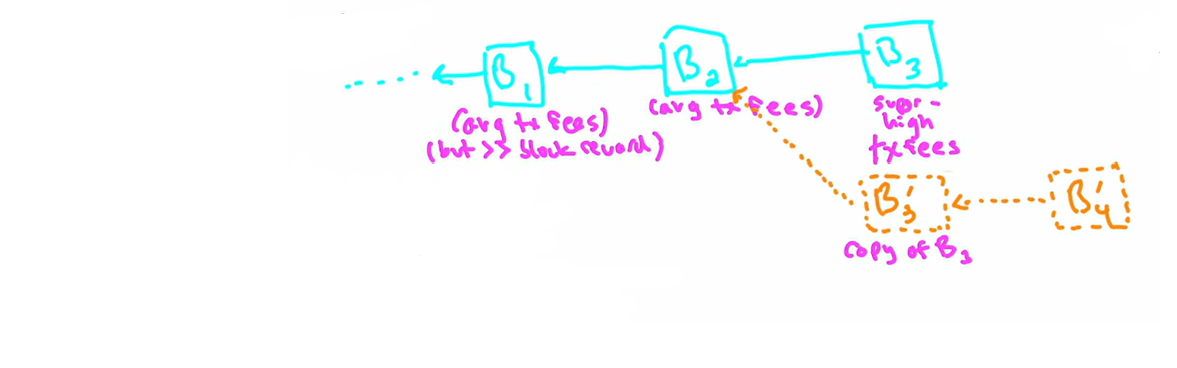
\includegraphics[scale = 0.8]{figures/f49.png}
    \caption{Large Transaction Fees: example}
    \label{fig:mesh1}
\end{figure}

\subsubsection{Implications}
Even with a small hash rate (1\% in the example), there can be situations where miners find it profitable to engage in selfish mining attacks if the transaction fees in a particular block are much higher than the average reward from a block.

\subsubsection{Addressing the Issue}
This situation raises concerns about the incentives provided to miners in the presence of large transaction fees. In the extreme case where multiple miners attempt selfish mining attacks to steal each other's rewards, progress in the blockchain could slow down significantly or even lead to a lack of liveness. Such issues are not currently prevalent in Bitcoin, it is essential to consider the future as block rewards are halved periodically. Over time, the dominance of transaction fees over block rewards may increase, potentially leading to increased incentives for selfish mining attacks.\\
As we mentioned, Ethereum's transition to EIP-1559 introduces a new transaction fee mechanism that mitigates the severity of selfish mining attacks. The mechanism involves burning some transaction fees, reducing the amount received by miners and, consequently, reducing the incentive for selfish mining attacks.


\section{Issues with First-Price Auctions}
In this section, we will discuss the new transaction fee mechanism proposed in EIP-1559 for Ethereum. Before delving into the details of how it works, we will first explore the need for an alternative to first-price auctions (FBAs) and the issues associated with them. Despite the success of FBAs in Bitcoin and Ethereum, there are significant challenges in figuring out how to bid optimally in such auctions.

\subsection{Challenges of First-Price Auctions}
First-price auctions are widely used in various application domains, including blockchain systems like Bitcoin and Ethereum. However, despite their prevalence, they come with significant challenges, particularly in the context of determining optimal bidding strategies. Let's delve into the main issues associated with first-price auctions and explore why they may not be the most suitable option for transaction fee mechanisms.

\subsubsection{Uncertainty of Competing Bids}
One of the primary difficulties in first-price auctions is the uncertainty surrounding the bids of other participants. Imagine you are a user who wants to include a transaction in a block, and the transaction fee is determined through a first-price auction. If you had telepathy and could magically know all the other participants' bids, your decision-making process would be straightforward. You could bid just high enough to outcompete others and secure a spot in the block. Unfortunately, in reality, this is not possible, and participants must make educated guesses about what their competitors might bid.

\subsubsection{Educated Guesses and Regretting Bids}
Making these educated guesses is no simple task, even for the most sophisticated individuals. Regardless of your intelligence and the quality of your guesses, there's always a chance that you will regret your bid in hindsight. For instance, consider the following scenarios:\\

\noindent
\textbf{Scenario 1: Bidding Too High}\\
You decide to bid a relatively high amount, hoping to secure your transaction's inclusion in the block. Eventually, your bid wins, and your transaction is added. However, upon reflection, you realize that you overpaid for the transaction to be included. In this case, you regret not having bid a lower amount.\\


\noindent
\textbf{Scenario 2: Bidding Too Low}\\
Alternatively, you may decide to bid conservatively, hoping to save on transaction fees. However, in doing so, you lose the bidding competition, and your transaction is excluded from the block. You discover that the bids were not as high as you initially assumed, and your conservative bidding strategy backfired. Consequently, you regret not having bid more aggressively.

\subsubsection{Automated Bidding and Its Limitations}
Some users opt to rely on software wallets that automate the bidding process based on recent bid data from the blockchain. While this is a step towards simplifying the process, it does not guarantee optimal bids. Users may still face frustration if their automated bids underestimate the optimal bid, leading to prolonged transaction confirmation times.

\subsubsection{User Experience on Public Blockchains}
Regular users of public blockchains like Ethereum often encounter issues with transaction fees and bid estimations. Users submit transactions through their wallets, which suggest appropriate bid amounts. However, due to the challenges mentioned earlier, there are instances where wallets underestimate the required bid, leading to delays in transaction confirmations. As a result, users may experience transaction hang times of significant duration, causing frustration and dissatisfaction.\\

The challenges of first-price auctions lie in the difficulty of optimally determining bid amounts without knowing the competing bids. This uncertainty can lead to regrets about both overpaying and underbidding, making the process less user-friendly and reliable. As a response to these challenges, Ethereum introduced the EIP-1559 mechanism, which aims to address these issues and create a more efficient and user-friendly transaction fee mechanism.

\subsection{Introducing EIP-1559}
The solution to the challenges of first-price auctions was proposed in Ethereum Improvement Proposal (EIP) 1559. This new mechanism introduced a fixed "base fee" that is automatically adjusted based on network demand. Users would now only need to include the base fee with their transactions, and the network would handle the rest.\\

With EIP-1559, the process of bidding on transaction fees became much simpler and more akin to the take-it-or-leave-it model of online shopping. Users no longer needed to make complex calculations or educated guesses about competing bids. Instead, they only needed to accept the prevailing base fee, which would be dynamically adjusted to reflect network conditions.\\

By adopting EIP-1559, Ethereum aimed to make the bidding process for transaction fees more user-friendly and efficient, reducing the frustration users faced with the old first-price auction mechanism. This change represented a significant step towards improving the overall user experience on the Ethereum network.

\subsection{Second Price Auctions (Vickery Auctions)}
In the context of alternatives to first-price auctions, we can name Second Price Auctions, also known as Vickery Auctions. These auctions offer a dominant strategy for bidders, meaning it is always in their best interest to bid their maximum willingness to pay.

\subsubsection{Dominant Strategy in Vickery Auctions}
In a Vickery Auction, the auction mechanism itself optimally shades the bids on behalf of the bidders, given the bids of all competitors. This means that a bidder should place the highest price they are willing to pay for an item, and the auction will automatically ensure they pay just one increment above the second-highest bid. As a result, bidders have no incentive to shade their bids, unlike in first-price auctions where bidders tend to bid less than their maximum willingness to pay to avoid overpaying.

\subsubsection{Comparison to First-Price Auctions}
While Second Price Auctions offer a straightforward bidding strategy, they are not suitable for blockchain applications like Bitcoin and Ethereum, specifically when it comes to transaction fees. The main issue is that these auctions rely on trusting the auctioneer or whoever runs the auction not to manipulate the price by injecting additional bids. In the case of blockchain, where miners have significant control over the blocks they produce, such manipulatability can lead to abuse and unfair practices.

\subsubsection{Inappropriateness for Blockchain Deployment}
Using Second Price or Vickery Auctions in the context of blockchain transaction fees would incentivize miners to create new transactions and include them in the block to boost their revenue from these auctions. This undermines the integrity of the blockchain system and is one of the reasons why such auction mechanisms are not used for determining transaction fees.\\
While Second Price Auctions offer an appealing dominant strategy for bidding, they are not a suitable solution for determining transaction fees in blockchains like Ethereum due to the potential for manipulation and abuse by miners. Instead, the EIP-1559 mechanism was introduced to provide an alternative that simplifies the bidding process while addressing the specific challenges faced in blockchain environments.

\section{EIP-1559}
In this section, we will explore the transaction fee mechanism proposed in EIP-1559, which was developed by Vitalik Buterin, the founder of Ethereum. The EIP stands for Ethereum Improvement Proposal. The new mechanism was introduced to address the drawbacks of first-price auctions, which were previously used for setting transaction fees in blockchain protocols like Bitcoin and early versions of Ethereum.\\

\noindent
\textbf{Intro.} First-price auctions were a natural choice for transaction fees in blockchain protocols. However, they had a significant drawback – it was challenging for users to bid intelligently in such auctions. This issue was highlighted by the fact that users needed to consider their competitors' bids and make educated guesses about them. Moreover, there was a constant risk of either overpaying for transaction inclusion or under-bidding and missing out on being included in a block. This contrasted sharply with a more familiar scenario like shopping on Amazon, where users could simply decide whether a product's price was acceptable to them and make a straightforward choice.\\

\noindent
\textbf{The Need for a Better Transaction Fee Mechanism:}\\
To illustrate this drawback further, imagine a first-price auction scenario in the blockchain context. Users would submit their bids for transaction fees, and the miner would select the transactions with the highest bids for inclusion in the block. However, since users do not have perfect information about their competitors' bids, they might end up bidding either too high or too low, leading to suboptimal outcomes.\\

For example, let's say there are three pending transactions, and users $A$, $B$, and $C$ submit bids of 20, 25, and 30 units of the native cryptocurrency, respectively. The miner, who is responsible for selecting the transactions for the block, chooses transaction $C$ with the highest bid of 30 units. However, in this scenario, if user $A$ had known that user B's bid was 25 units, they could have bid 26 units to get their transaction included instead. Similarly, if user $C$ had known about user A's bid, they might have bid just enough to outbid user $A$, say 21 units. In this way, the first-price auction mechanism leads to a lack of transparency and suboptimal outcomes for users.\\

This issue becomes even more challenging when considering the dynamic nature of transaction fees in a blockchain. As the number of transactions and the network's demand fluctuates, so do the fees. Users have to constantly adapt to changing conditions and make guesses about other users' behavior to bid effectively.

The desire for a more user-friendly and predictable transaction fee mechanism, akin to shopping on Amazon, led to the development of the transaction fee mechanism proposed in EIP-1559.\\
EIP-1559 introduces the concept of a base fee, which serves as a reserve price or minimum bid for transaction inclusion in a block. Transactions with bids lower than the base fee are considered invalid and cannot be included in the block. This base fee is denominated in units of the native cryptocurrency, making it easy for users to understand. Additionally, users have the option to bid higher than the base fee if they wish to increase their chances of inclusion in a block.\\

The key idea behind EIP-1559 is to make the fee mechanism more transparent and user-friendly. Users no longer have to worry about outbidding their competitors or making complex decisions based on incomplete information. Instead, they can focus on whether the base fee is acceptable to them, just like a straightforward take-it-or-leave-it offer. This simplicity and predictability bring the user experience closer to that of shopping on Amazon, where users can decide whether a product's price is worth it to them without the need for complex calculations or competition analysis.\\

\nt{
\begin{center}
    \textbf{Key Idea \#1}
\end{center}
Each block has a base free $r > 0$(reserve price)
\begin{itemize}
    \item minimum bid to be eligible for inclusion (it's okay to bid more)
    \item Deterministic (protocol-computed) function of predecessor blocks (can vary with the block)
\end{itemize}}
The mechanism's success lies in the combination of the base fee and the fee-burning aspect. By burning the base fee revenues instead of passing them on to the miner, collusion between users and miners becomes ineffective. This ensures that users cannot manipulate the system to their advantage and promotes fair and efficient transaction inclusion.

\subsection{Determining the Base Fee}
The base fee is a critical component of the transaction fee mechanism proposed in EIP-1559. It acts as a reserve price or minimum bid for transaction inclusion in a block. Any transaction with a bid lower than the base fee is considered invalid and cannot be included in the block. This ensures that all transactions included in a block meet a minimum fee requirement.\\

The base fee is denominated in units of the native cryptocurrency, which makes it easy for users to understand the minimum fee they need to pay for their transactions to be eligible for inclusion.

\subsubsection{Deterministic Computation}
One essential characteristic of the base fee is that it is protocol-computed. This means that it is not suggested by users like in first-price auctions. Instead, the base fee is determined entirely by the protocol, based on the history of past blocks. It is a deterministic function of everything that has happened leading up to the current block. The contents of the current block do not influence the computation of the base fee.\\
This deterministic computation ensures that the base fee remains objective and transparent. Users do not have to worry about subjective biases or manipulations in setting the base fee. It is purely based on historical data and is uniquely determined by past events.

\subsubsection{Variability with Blocks}
The base fee is not fixed but can vary from block to block. As the blockchain's demand and transaction volume fluctuate, the base fee can adjust accordingly. For example, if there is a surge in network activity, the base fee might increase to incentivize miners to include more transactions in the block. Conversely, during periods of lower activity, the base fee may decrease to reflect the reduced demand.\\
This variability helps the mechanism adapt to changing network conditions and ensures that the transaction fee system remains efficient and responsive to demand fluctuations.

\subsubsection{Example of Base Fee Adjustment}
To illustrate the concept of base fee variability, let's consider a hypothetical example. Suppose the blockchain has been operating with a base fee of 100 units of the native cryptocurrency for several blocks. However, due to increased network activity and demand, the protocol computes the base fee for the next block to be 120 units.\\
In this scenario, any transaction with a bid lower than 120 units will be considered invalid and ineligible for inclusion in the next block. Users who want their transactions to be included must bid at least 120 units, which becomes the minimum bid for this specific block.\\
Conversely, in the subsequent block, if the network activity decreases, the protocol might adjust the base fee to 90 units. Now, transactions with bids lower than 90 units will be invalid for inclusion in that block.\\
This dynamic adjustment of the base fee based on network conditions ensures that the transaction fee mechanism remains responsive and efficient, promoting optimal transaction inclusion in blocks.\\

\subsection{Destination of Base Fee Revenues}
In the context of EIP-1559, the destination of base fee revenues plays a crucial role in determining the effectiveness of the transaction fee mechanism. Initially, it may seem reasonable to direct the base fee revenues to the miner of the block, just like in first-price auctions. After all, the miner is the one who decides which transactions to include in their block, so it makes sense to reward them with transaction fees.

However, the text highlights a key problem with this approach. If the base fee revenues are passed on to the miner, it essentially renders the base fee useless. Users and miners could potentially collude to avoid paying the base fee and manipulate the system to their advantage.\\

To illustrate this issue, let's consider the following example:
\ex{The base fee ($r$) is set at 100 units of the native currency. Now, imagine there are several pending transactions, and all of them are only willing to pay up to a maximum of 50 units as their bid. In this scenario, if all participants act honestly, they would bid at most $r/2$, i.e., 50 units, since that is what they are willing to pay.\\
In a scenario where the base fee is not burned, users and the miner could potentially collude to manipulate the system and pay less than the base fee while still getting their transactions included.

In this collusion scenario, users would publicly bid $r$ (the base fee) for their transactions on-chain, making it seem like they are willing to pay the full base fee. However, they would privately communicate with the miner through a side channel, indicating that they are only willing to pay $b_i$, for instance here, 45 (less than the base fee). The miner, being part of this collusion, would include all these transactions in the block, collecting the base fee of 100 from each of them. Off-chain, the miner would then refund the difference $r - b_i$ for example here (100 - 45 = 55) back to the users, essentially nullifying the base fee.\\

As a result, none of the pending transactions would be eligible for inclusion in the block, and the miner would be forced to produce an empty block. While the miner would still collect the block reward, they would not receive any transaction fee revenue, leading to an undesirable outcome for both users and miners.\\

To circumvent this situation and achieve better game theoretic properties, EIP-1559 proposes an alternative approach for the destination of base fee revenues: fee burning. Instead of rewarding the miner with the base fee revenues, the mechanism simply burns the fees by sending them to a null address, effectively taking those coins out of circulation forever.}\\
This fee-burning process helps offset the inflation caused by block rewards. In the example given earlier, when some transaction fees are burned, the effective inflation rate of the native currency decreases from 4\% to 2\%. This means that the value of the native currency held by users is being devalued at a slower rate, providing a financial benefit to all holders.\\
As a result, the fee-burning aspect of EIP-1559 became a significant selling point for the proposed transaction fee mechanism. It not only addressed the issue of collusion but also presented an opportunity for users to benefit from a reduction in the effective inflation rate, making it appealing to the Ethereum community and gaining widespread support. By opting for fee burning instead of rewarding the miner, the mechanism ensures better game theoretic properties and provides financial benefits to all holders of the native currency.

\subsection{Excess Transaction Fees}
In the new transaction fee mechanism introduced by EIP-1559, users have the option to bid more than the base fee if they wish to increase the chances of their transactions being included in a block. The base fee acts as the minimum bid necessary for eligibility, but any higher bid is also considered for inclusion.\\

Let's revisit the previous example of collusion between users and miners, where users bid the base fee on-chain but privately communicate to the miner their willingness to pay a lower amount. In this case, the miner includes all transactions with the on-chain bid of the base fee, making them eligible for inclusion. However, since the base fee is not transferred to the miner, they cannot provide refunds off-chain. Therefore, this type of collusion becomes ineffective, and all transactions remain eligible, defeating the purpose of the base fee.\\
On the other hand, in the presence of honest transactions that bid more than the base fee, the excess transaction fees above the base fee are indeed transferred to the miner of the block. This ensures that miners are incentivized to include transactions with higher fees, as they will receive additional revenue for doing so.\\

The ability for users to bid more than the base fee allows for greater flexibility in transaction pricing. For example, if a user urgently needs their transaction to be included quickly, they can bid a higher fee to prioritize their transaction over others. Conversely, users with less urgency can choose to bid closer to the base fee to save on transaction costs.\\

Incorporating excess transaction fees into the mechanism ensures that the base fee does not discourage users from providing higher fees when they find it necessary or beneficial. This way, the mechanism strikes a balance between predictable pricing through the base fee and market-driven pricing with the inclusion of excess fees.\\

It's worth noting that this combination of base fee, fee burning, and excess transaction fees provides a more efficient and user-friendly transaction fee mechanism compared to traditional first-price auctions. The mechanism incentivizes miners to include transactions with higher fees while reducing the overall inflation rate through fee burning. This aspect of EIP-1559 garnered significant support from the Ethereum community, making it a prominent reason for the adoption of the new transaction fee mechanism.

\subsection{OCA Proofness Property}
\thm{}{Miner-user collusion no longer helps.}
The Off-Chain Agreement (OCA) proofness property is a critical aspect of the EIP-1559 transaction fee mechanism. It ensures that collusion between users and miners does not lead to any advantages for them, and they cannot manipulate the mechanism off-chain to gain better outcomes than honest participation on-chain.\\

To better understand the significance of OCA proofness, let's revisit the example of collusion that was mentioned earlier. Suppose we have a block with a base fee of $r$, set at 100. There are several pending transactions, and all of them are willing to pay up to a maximum of 50. In a scenario where the base fee is not burned, users and the miner could collude to game the system and pay less than the base fee while still getting their transactions included.\\

In the collusion scenario, users would publicly bid $r$ (the base fee) for their transactions on-chain, but they would inform the miner privately through a side channel that they are only willing to pay 45 (less than the base fee). The miner, in turn, would include all these transactions in the block, collecting the base fee of 100 from each of them. Off-chain, the miner would then refund the difference (100 - 45 = 55) back to the users, essentially nullifying the base fee.\\

However, with the OCA proofness property in EIP-1559, this collusion strategy proves to be ineffective. The key reason behind this is that the base fee revenues are burned instead of being passed on to the miner. As a result, the miner is not in a position to refund the users since any refund would be an out-of-pocket expense.\\

In a more general context, the OCA proofness property ensures that no matter what strategies users and miners employ off-chain, they cannot achieve better outcomes than if they participate honestly on-chain. Any attempts to manipulate the mechanism by shading bids, sharing information, or collusion are futile, as the protocol's rules are designed to prevent such efforts.\\

By satisfying the OCA proofness property, EIP-1559 ensures fairness, transparency, and predictability in the transaction fee mechanism. Users can confidently bid based on their willingness to pay, knowing that the mechanism cannot be exploited or influenced by off-chain agreements.

\section{What should the Base fee Be?}

\subsection{Ideal Base Fee: Market Clearing Price}
The ideal base fee, from an economic efficiency standpoint, would be a \textit{market clearing price}. In this context, a market clearing price refers to a base fee that is set at a level where the subset of pending transactions willing to pay this fee would exactly fill up a block, neither more nor less.

To understand why a market clearing price is considered the best base fee, let's examine the advantages it offers:

\begin{enumerate}
    \item \textbf{100\% Utilization:} Setting the base fee at the market clearing price ensures that the blockchain's capacity is fully utilized. All available block space is occupied by transactions, maximizing the usage of this scarce resource, which is the blockchain.
    \item \textbf{Highest Value Transactions:} The transactions included in the block under a market clearing price are precisely the ones willing to pay this fee. As a result, only the highest-value transactions are included, prioritizing those that offer the most significant value to users.
\end{enumerate}

Consider this example: 
\ex{If a magical base fee of 50 units fell from the sky, and there are pending transactions willing to pay up to 50 units, then exactly the right number of transactions to fill up the block would be included. Any additional transactions would be excluded because they are not willing to pay the base fee, and any fewer transactions would indicate that some available block space is unused.}

This concept of a market clearing price aligns with the notion of economic efficiency, where the scarce resource (block space in this case) is utilized optimally and allocated to the highest value transactions. It ensures that the blockchain operates at its full potential, and only the most valuable transactions get included.\\

A base fee set higher than the market clearing price would be inefficient because the block would not be completely full. In this scenario, the number of transactions willing to pay the higher base fee may not be sufficient to fill up the entire block. On the other hand, setting the base fee lower than the market clearing price would lead to inefficiencies as low-value transactions and high-value transactions would be on equal footing, potentially occupying valuable block space. Therefore, the market clearing price is an important benchmark for the ideal base fee, as it ensures both optimal resource utilization and prioritization of valuable transactions, ultimately contributing to economic efficiency on the blockchain.

\section{Computing the Base Fee: Variable Size Blocks}
Computing the Base Fee in Ethereum's EIP-1559 is done using the concept of \textbf{Variable Size Blocks}. This approach allows for the automatic adjustment of the base fee based on the previous block's utilization, which helps to maintain a market clearing price for transactions.

\noindent
\textbf{Variable Size Blocks Explained:}
Traditionally, blockchains have had a hard cap on block size, where each block must not exceed a certain size (e.g., 15 million units of gas). This was done to ensure that all nodes in the network can keep up with the processing of transactions and to maintain minimal computational and storage requirements for running the protocol.\\
However, EIP-1559 introduces a different approach by introducing a \textit{target block size}. Instead of strictly adhering to a fixed block size cap, the protocol allows for some flexibility. The target block size is set as the desired average size of blocks and is used to bind the block size on average.

\nt{
\begin{center}
    \textbf{Key Idea \#2}
\end{center}
Allow variable size blocks (i.e relax per-block hard cap)
\begin{itemize}
    \item[$-$] Per-block size constraint overkill, the average-size constraint should be good enough
    \item[$-$] Set target block size $C$
    \item[$-$] Allow blocks of size up to $2C$ (borrow capacity from the near future)
\end{itemize}}

\noindent
\textbf{Example of Target Block Size:}
In Ethereum, if the target block size is set to 15 million units of gas, the average size of blocks should ideally be around this value.\\

\noindent
\textbf{Adjusting the Block Size:}
The EIP-1559 allows for violations of the target block size within certain limits. In Ethereum, blocks are allowed to be double the target block size, i.e., up to 30 million units of gas.\\

\noindent
\textbf{Benefits of Variable Size Blocks:}
The introduction of variable-size blocks offers several advantages:
\begin{itemize}
    \item \textit{Flexibility:} The blockchain can adapt to periods of high demand by borrowing space from the future, allowing it to handle sudden spikes in transaction volume.
    \item \textit{Efficiency:} The blockchain can optimize block space allocation, ensuring that it remains close to its target block size, leading to more efficient resource utilization.
\end{itemize}

\noindent
\textbf{Local Search for Base Fee Adjustment:}
The variable size blocks enable the implementation of the local search approach to adjust the base fee. 
\begin{itemize}
    \item If the previous block's size is less than the target block size (an \textit{empty block}), it indicates that the base fee is too high, as there weren't enough eligible transactions to fill the block. In this case, the base fee is decreased by 12.5\% for the next block.
    \item On the other hand, if the previous block's size is double the target block size (a \textit{double full block}), it means there is excess demand at the current base fee level, and the base fee should be increased. Therefore, the base fee is increased by 12.5\% for the next block.
    \item For block sizes that are between the empty and double full conditions, the base fee adjustment is done through \textit{linear interpolation}. This ensures a smooth and gradual adjustment of the base fee based on the deviation from the target block size.
\end{itemize}

\noindent
\textbf{Example of Base Fee Adjustment:}
Let's say the target block size is 15 million units of gas. If a block has a size of 12 million units of gas (less than the target), the base fee for the next block will be decreased. Conversely, if a block has a size of 30 million units of gas (double the target), the base fee for the next block will be increased.\\

Variable size blocks play a crucial role in the EIP-1559 transaction fee mechanism, enabling automatic adjustment of the base fee based on the actual demand for block space. By borrowing space from the future when necessary, the mechanism achieves efficient resource utilization and maintains a market clearing price, making it a powerful and user-friendly solution for transaction fee computation in Ethereum.

\section{Excessively Low Base Fees}
Up till now, we discussed first-price auctions and their drawbacks. It is challenging to determine how to bid in such auctions, requiring significant cognitive effort. This led to the introduction of the new transaction fee mechanism proposed in EIP-1559, which Ethereum switched to in early August 2021. The mechanism involves a burned base fee and a local search procedure to adjust the base fee over time. To accommodate sudden spikes in demand, variable-sized blocks were introduced, with a target average block size of $C$ and a hard per-block cap of $2C$.

\subsection{Two Regimes of the Transaction Fee Mechanism}
The transaction fee mechanism proposed in EIP-1559 exhibits two distinct regimes that determine how easy it is for users to figure out how to bid in the Ethereum network.

\dfn{}{A block's base fee $r$ is \textit{excessively low} if the total size of all pending eligible (i.e, $\text{bid} \geq r$) transactions is $> 2C (\text{size of a double-full block})$}

\subsubsection{Regime 1: Base Fee Not Excessively Low}
In this first regime, the base fee is not excessively low, and there is enough room in the blocks to accommodate all eligible transactions without competition. Bidding in this regime is as simple as shopping on Amazon. Users can estimate the appropriate fees by just bidding the base fee ($r$) or adding a small tip ($\Delta$) to incentivize miners to include their transactions.

\thm{}{If base fee $r$ is not excessively low, it's optional to bid $r$ (or maby $r \times s$ for a small $s$) so that miners incentivized to include $tx$s rather than produce empty blocks. [Otherwise, reverts to a first-prize auction]}
We can use this scenario to go shopping on Amazon, where products have a posted price, and users can take it or leave it. Similarly, in this regime, the blockchain offers a take it or leave it deal for transaction inclusion. Users can bid the base fee or add a tip if they wish, but there is no need for aggressive bidding or complex strategies because there is enough capacity to include all transactions.\\
Additionally, the excess between the bid and the base fee is burned, meaning that if a user bids more than the base fee, the additional amount is transferred to the miner, and the base fee itself is burned.\\

This regime is the more common one and is characterized by blocks that are not double full, indicating sufficient space for all eligible transactions. In practice, it is observed that most blocks fall under this regime, providing a straightforward bidding experience for users.

\subsubsection{Regime 2: Base Fee Excessively Low}
In the second regime, the base fee becomes excessively low, meaning that there is not enough space in the blocks to accommodate all eligible transactions. This situation occurs less frequently, but it does happen in specific scenarios.

When the base fee is excessively low, miners must choose which transactions to include in the limited block space, akin to a first-price auction. This creates a situation where users have to compete with each other through their bids to have their transactions included in the block.

In this regime, the excess between the bid and the base fee is once again burned, but the miner receives the burned amount. As a result, the miner has an incentive to prioritize transactions with higher bids to maximize their share of the transaction fee.\\
While this situation does arise occasionally, it is not as problematic as traditional first-price auctions. The EIP-1559 mechanism still provides improvements, as the base fee is burned, reducing the risk of strategic manipulation, and there are fewer scenarios where users need to compete intensely.

\subsection{Determining the Regime}
The determining factor for the regime is whether the current base fee ($r$) is excessively low or not. If the total size of eligible transactions at that base fee exceeds $2C$, it is considered excessively low. Moreover, if it exceeds $C$, it is already too low, indicating a need to increase it.\\


\subsection{Factors Affecting the Regime}
Now the important question is, Why might the base fee be excessively low??\\
The regime, which determines whether the transaction fee mechanism behaves as a posted price mechanism (good regime) or a first-price auction (bad regime), can be influenced by the following factors:

\subsubsection{Sudden Increases in Demand}
One of the factors that can lead to the bad regime is sudden sharp increases in demand for the blockchain. These spikes in demand often occur during events such as major NFT drops on Ethereum. When the demand for transactions surges, the market clearing price can rise significantly. However, due to the design of the transaction fee mechanism in EIP-1559, the adjustment of the base fee is limited by the protocol.\\

The local search procedure used in EIP-1559 aims to find the market clearing price with respect to a normal block size ($C$). However, if there is a sudden increase in demand, the market clearing price can quickly jump to a higher level, exceeding the current base fee ($r$). As a result, the base fee might be too low to accommodate all the eligible transactions, causing the regime to shift to the bad regime.\\

During this transitory period, which may last for several minutes, the base fee has not yet caught up with the higher market clearing price. As a consequence, miners may find themselves with an excessively low base fee for a short period, leading to competition among transactions and a first-price auction-like behavior.

\subsubsection{Random Variability in Block Production}
Another factor that can impact the regime is the random variability in block production, or in other words, unusually long period of time between consecutive blocks, which is characteristic of Ethereum's proof-of-work implementation. While the average block production time is around 13 seconds, it is not precise and can vary. Miners must solve a cryptographic puzzle to produce a block and sometimes it can take longer than usual to find a valid solution.\\

When blocks take longer to produce than expected, more eligible transactions can accumulate during that time. This can lead to a situation where there are more transactions than the base fee ($r$) can accommodate, pushing the regime to the bad regime. For example, if the base fee was set to handle the average block production time (13 seconds), but a block takes double the expected time (26 seconds), there will be three times as many eligible transactions as anticipated. This sudden increase in the number of eligible transactions can exceed the capacity of the current base fee, resulting in the regime shifting to the bad regime.

\subsection{Future Predictions}
Currently, based on data from \url{watchtheburn.com}, the good regime (base fee not excessively low) is more prevalent than the bad regime (base fee excessively low). It is estimated that the good regime occurs around 90\% of the time. However, it is worth noting that Ethereum is planning to switch to a proof-of-stake design in 2022. With proof of stake, the random variability in block production will be reduced since blocks will be produced more regularly, approximately every 12 seconds. As a result, the second culprit, random block time variability, will have less influence on the regime.\\

After the switch to proof of stake, it is expected that the good regime will become even more prevalent, occurring around 95\% of the time, with the bad regime becoming less frequent. Nevertheless, the occasional sudden spikes in demand will still lead to transitory periods where the base fee might temporarily be excessively low.

\section{Pros and Cons of Burning Fees}
\subsection{Consequences of Burning Base Fee Revenues}
The burning of base fee revenues in the EIP-1559 proposal has multiple implications, impacting both miners and holders of the native currency, such as Ethereum. Let's delve into the consequences of this design choice:

\subsubsection{Benefiting Holders of Native Currency}
By burning the coins used to pay the base fee, these coins are permanently removed from circulation. This reduction in the coin supply has significant implications for the holders of the native currency. In analogy to the equities world, this process resembles stock buybacks, which, in principle, should raise the value of all remaining shares in circulation.\\

To understand this better, let's consider a scenario with a fixed market capitalization for Ethereum. In such a case, the market capitalization should ideally be independent of the number of coins in circulation and dictated by factors like the demand for the currency and speculation about its future market cap.\\

Now, imagine cutting the supply of circulating coins in half while keeping all other factors constant. With a fixed market capitalization, each remaining coin would have to be priced twice as much to compensate for the halved supply. This intuition illustrates why burning base fee revenues benefits the remaining holders of the native currency. As coins are taken out of circulation, the value of the remaining coins should increase, potentially leading to price appreciation.

\subsubsection{Effect on Inflation Rate}
As mentioned in the text, the burning of base fee revenues has the aggregate effect of reducing the inflation rate of Ethereum. Prior to EIP-1559, Ethereum's inflation rate was roughly four percent. However, with the implementation of the new transaction fee mechanism, the inflation rate has decreased to approximately 2\%.\\

This reduced inflation rate benefits all holders of the native currency, as the pace of coin issuance is slowed down. By not printing coins as rapidly as before, the switch to the transaction fee mechanism should be favorable to all holders of Ethereum, allowing them to benefit from potentially increased coin value.

\subsubsection{Impact on Miners' Revenue}
While the burning of base fee revenues does result in a loss of revenue for miners, the consequences may not be as catastrophic as initially perceived. In the post-EIP-1559 world, miners still have multiple revenue streams at their disposal:

\begin{enumerate}
    \item \textbf{Block Rewards}: Miners receive two new ethers for every block they successfully mine. This block reward serves as a steady income stream for miners.
    
    \item \textbf{Excess Bid Fees}: Users have the option to bid above the base fee for their transactions. Any amount exceeding the base fee is transferred to the miner. Therefore, miners can still earn additional revenue through these excess bids in a post-EIP-1559 world.
    
    \item \textbf{Special Treatment Transactions}: Certain transactions may require special treatment, such as being included as the first transaction in a block. Users may offer higher fees to incentivize miners to prioritize their transactions. This can result in a significant source of additional revenue for miners.

    \item \textbf{Miner Extractable Value (MEV)}: Miner Extractable Value is a unique source of revenue for miners that involves inspecting the content of transactions and potentially optimizing block inclusion to their advantage. This can be especially significant in decentralized finance (DeFi) transactions, where miners can profit from various opportunities.
\end{enumerate}
Despite the loss of base fee revenues, miners retain multiple avenues to generate income, which can soften the impact of the transition to the new fee mechanism.\\

In conclusion, while the burning of base fee revenues does have consequences for miners and holders of the native currency, it may not be as detrimental as initially anticipated. The reduced inflation rate benefits all holders of the currency, potentially leading to increased coin value. Additionally, miners can still rely on block rewards, excess bid fees, special treatment transactions, and Miner Extractable Value to maintain revenue in the post-EIP-1559 world. Overall, the Ethereum community successfully navigated the implementation of this major update, showcasing the decentralized decision-making process and resilience of the network.

\subsection{Impact on Miners and Blockchain Security}
The implementation of EIP-1559, specifically the burning of base fee revenues, has significant implications for miners and the overall security of the Ethereum blockchain.

\subsubsection{Decreased Miner Revenue}
With the introduction of the transaction fee mechanism in EIP-1559, miners experience a decrease in their revenue. While the base fee revenues are no longer directly passed on to miners, they still receive block rewards, excess bid fees, and revenue from special treatment transactions and Miner Extractable Value (MEV). However, the reduction in base fee revenues impacts the overall miner profitability.

To understand this impact better, let's consider an example where a miner is barely covering their operating costs with their previous revenue stream. The decrease in revenue due to the burned base fee revenues might result in a situation where their income is significantly lower, say around 20-30\%. In such a scenario, the miner may choose to stop mining altogether to avoid losses. However, it is important to note that the decrease in revenue is not as catastrophic as it may initially seem. Some miners might continue to find mining profitable due to the other revenue streams, and the decrease in hash rate can create a feedback loop that affects mining difficulty and rewards.

\subsubsection{Feedback Loop on Mining Difficulty}
As some miners exit the network due to decreased profitability, the overall hash rate of the Ethereum network decreases. The difficulty adjustment algorithm in proof-of-work blockchains, like Ethereum, ensures that blocks are produced at a consistent rate (e.g., one block every 13 seconds).\\

Suppose a miner chooses to remain in the network despite the decreased revenue. Since the hash rate has reduced, the cryptographic puzzles become easier to solve. As a result, each hash attempt is more likely to yield a solution, leading to more frequent block mining for the remaining miners.\\
This feedback loop tends to stabilize the network to a new equilibrium where the remaining miners find it more profitable to mine despite the decrease in base fee revenues. The adjustment in mining difficulty maintains the block production rate, which is crucial for the proper functioning of the Ethereum blockchain.

\subsubsection{Blockchain Security Concerns}
One potential concern arising from the decrease in hash rate is the impact on the security of the Ethereum blockchain. A lower hash rate makes the network more susceptible to 51\% attacks, where an attacker gains control of a majority of the network's computing power.\\
A successful 51\% attack would allow the attacker to manipulate transactions, double-spend coins, and disrupt the network's integrity. The burning of base fee revenues may lead to some miners exiting the network, making it easier for potential attackers to acquire the necessary hash rate for a 51\% attack. However, it is worth noting that this concern was not a significant sticking point during the discussions around EIP-1559 in the Ethereum community. Many leaders in the community believed that the remaining block rewards would provide sufficient incentives for miners to maintain network security.\\

In retrospect, the Ethereum network's security has not been severely compromised following the implementation of EIP-1559. While the decrease in hash rate can be a potential concern, the network has continued to operate securely with miners adapting to the new economic model.\\

Overall, the impact of EIP-1559 on miners and blockchain security was a major point of discussion in the Ethereum community. Despite the decrease in miner revenue, the network has demonstrated resilience, and the feedback loop on mining difficulty has contributed to maintaining network security.\\

The implementation of EIP-1559 sparked extensive discussions within the Ethereum community, with varying perspectives on its impact on miners and overall network security. Despite the decrease in miner revenue, the community managed to successfully deploy this major update in a decentralized and distributed manner. In the next chapter, we will explore proof-of-stake blockchains as an alternative to proof-of-work, focusing on their significance and benefits.
